
% ----------------------------------------------------------------------
%  Set the document class
% ----------------------------------------------------------------------
\documentclass[11pt,a4paper,twoside]{article}

% ----------------------------------------------------------------------
% Define external packages, language, margins, fonts and new commands
% ----------------------------------------------------------------------
%\input{preamble} 
\usepackage[utf8]{inputenc}   % <<<<< Linux
\usepackage[english]{babel} % <<<<< English
\usepackage{notoccite}
\usepackage[skip=0.5\baselineskip]{caption}
\hyphenation{GTKWave}
\usepackage{listings}
\usepackage[all]{nowidow}
\usepackage{float}
%blind text
\usepackage{lipsum}
\usepackage{amsmath} 
\usepackage{graphicx}
\graphicspath{ {./} {../../figlib/} }
\def\FontLn{% 16 pt normal
  \usefont{T1}{phv}{m}{n}\fontsize{16pt}{16pt}\selectfont}
\def\FontLb{% 16 pt bold
  \usefont{T1}{phv}{b}{n}\fontsize{16pt}{16pt}\selectfont}
\def\FontMn{% 14 pt normal
  \usefont{T1}{phv}{m}{n}\fontsize{14pt}{14pt}\selectfont}
\def\FontMb{% 14 pt bold
  \usefont{T1}{phv}{b}{n}\fontsize{14pt}{14pt}\selectfont}
\def\FontSn{% 12 pt normal
  \usefont{T1}{phv}{m}{n}\fontsize{12pt}{12pt}\selectfont}

% Use Arial font as default
%
\renewcommand{\rmdefault}{phv}
\renewcommand{\sfdefault}{phv}
\usepackage{geometry}	
\geometry{verbose,tmargin=2.5cm,bmargin=2.5cm,lmargin=2.5cm,rmargin=2.5cm}

%\usepackage{setspace}
%\renewcommand{\baselinestretch}{1.5}

\usepackage[pdftex]{hyperref} % enhance documents that are to be
                              % output as HTML and PDF
\hypersetup{colorlinks,       % color text of links and anchors,
                              % eliminates borders around links
%            linkcolor=red,    % color for normal internal links
            linkcolor=black,  % color for normal internal links
            anchorcolor=black,% color for anchor text
%            citecolor=green,  % color for bibliographical citations
            citecolor=black,  % color for bibliographical citations
%            filecolor=magenta,% color for URLs which open local files
            filecolor=black,  % color for URLs which open local files
%            menucolor=red,    % color for Acrobat menu items
            menucolor=black,  % color for Acrobat menu items
%            pagecolor=red,    % color for links to other pages
            pagecolor=black,  % color for links to other pages
%            urlcolor=cyan,    % color for linked URLs
            urlcolor=black,   % color for linked URLs
	          bookmarks=true,         % create PDF bookmarks
	          bookmarksopen=false,    % don't expand bookmarks
	          bookmarksnumbered=true, % number bookmarks
	          pdftitle={report},
            pdfauthor={Andre C. Marta},
%            pdfsubject={Thesis Title},
%            pdfkeywords={Thesis Keywords},
            pdfstartview=FitV,
            pdfdisplaydoctitle=true}

\usepackage[numbers,sort&compress]{natbib} % <<<<< References in numbered list [1],[2],...
\usepackage{subcaption} 
\usepackage{mdframed}

%%%%%%%%%%%%%%%%%%%%%%%%%%%%%%%%%%%%%%%%%%%%%%%%%%%%%%%%%%%%%%%%%%%%%%%%
%     Begin Document                                                   %
%%%%%%%%%%%%%%%%%%%%%%%%%%%%%%%%%%%%%%%%%%%%%%%%%%%%%%%%%%%%%%%%%%%%%%%%


\begin{document}

% Set plain page style (no headers, footer with centered page number)
\pagestyle{plain}

% Set roman numbering (i,ii,...) before the start of chapters
%\pagenumbering{roman}

% ----------------------------------------------------------------------
%  Cover page
% ----------------------------------------------------------------------
%%%%%%%%%%%%%%%%%%%%%%%%%%%%%%%%%%%%%%%%%%%%%%%%%%%%%%%%%%%%%%%%%%%%%%%%
%                                                                      %
%     File: Thesis_FrontCover.tex                                      %
%     Tex Master: Thesis.tex                                           %
%                                                                      %
%     Author: Andre C. Marta                                           %
%     Last modified :  2 Jul 2015                                      %
%                                                                      %
%%%%%%%%%%%%%%%%%%%%%%%%%%%%%%%%%%%%%%%%%%%%%%%%%%%%%%%%%%%%%%%%%%%%%%%%

\thispagestyle {empty}

% IST Logo - Signature A
% parameters: bb=llx lly urx ury (bounding box), width=h_length, height=v_length, angle=angle, scale=factor, clip=true/false, draft=true/false. 
\includegraphics[bb=9.5cm 11cm 0cm 0cm,scale=0.29]{IST_A_CMYK_POS}

\begin{center}
%
% Figure (Image or plot)
\vspace{1.0cm}
% height = 50 mm
%\includegraphics[height=50mm]{Figures/Airbus_A350.jpg}

% Title, author and degree
\vspace{1cm}
{\FontLb Circuit Theory and Electronics Fundamentals} \\ % 
\vspace{1cm}
{\FontSn Engineering Physics} \\ % <<<<< EDIT COURSE
\vspace{1cm}
{\FontSn Lab 5: Bandpass filter using OPAMP} \\
\vspace{1cm}
{\FontSn Beatriz Rosalino (96514), Mariana Ribeiro (96552), Sofia Guerreiro (96567)} \\
\vspace{1cm}
{\FontSn 6 June, 2021} \\ % <<<<< EDIT DATE (corresponds to date of oral examination)
%
\end{center}



% ----------------------------------------------------------------------
% Dedication page (optional)
% ----------------------------------------------------------------------
%\input{dedication} 
%\cleardoublepage

% ----------------------------------------------------------------------
%  Acknowledgments (optional)
% ----------------------------------------------------------------------
%\input{acknowledgements}
%\cleardoublepage

% ----------------------------------------------------------------------
%  Abstract (both in English and Portuguese)
% ----------------------------------------------------------------------
%\input{resumo} 
%\cleardoublepage

%\input{abstract} 

% ----------------------------------------------------------------------
%  Table of contents, list of tables, list of figures and nomenclature
% ----------------------------------------------------------------------

% Table of contents
%
\tableofcontents

% List of tables
%\addcontentsline{toc}{section}{\listtablename}
%\listoftables
%\cleardoublepage 

% List of figures
%\addcontentsline{toc}{section}{\listfigurename}
%\listoffigures
%\cleardoublepage 

% Set arabic numbering (1,2,...) after preface
%
%\setcounter{page}{1}
%\pagenumbering{arabic}

% ----------------------------------------------------------------------
%  Body
% ----------------------------------------------------------------------

\section{Introduction}
\label{sec:intro}
The main goal of this work is to analyze an RC circuit and study its various responses to a voltage source that changes over time. First, we studied the behavior of the circuit when the voltage imposed on the capacitor was constant and non zero (Section ~\ref{ssec:tl}), then we studied the natural response of the capacitor (voltage source imposing voltage equal to 0) in (Section ~\ref{ssec:n}), the forced response (voltage source imposing sinusoidal voltage) in (Section ~\ref{ssec:fs}), over time. We also studied the circuit for different frequencies of the sinusoidal signal, plotting the voltages at the capacitor and the nodes of its terminals as functions of frequency Section ~\ref{ssec:freq}.\\

Our circuit (Figure ~\ref{fig:circuit}) consists of 7 resistors, 2 voltage sources - 1 independent, and 1 current controlled dependent one, 1 independent current source and 1 capacitor.\\
The voltage provided by the independent source follows the equation:
\begin{equation}\label{eqn:vss}
\begin{split}
{v_s (t)} = \left\{\begin{array}{ll} \ V_s ,  \quad \ \  if \ \  \ t \leq 0 \\ 
 \ sin(2 \pi f t) , \quad \ \  if \ \ \ t \textgreater 0 \end{array} \right.
  \end{split}
\end{equation}
\begin{figure}[H] \centering
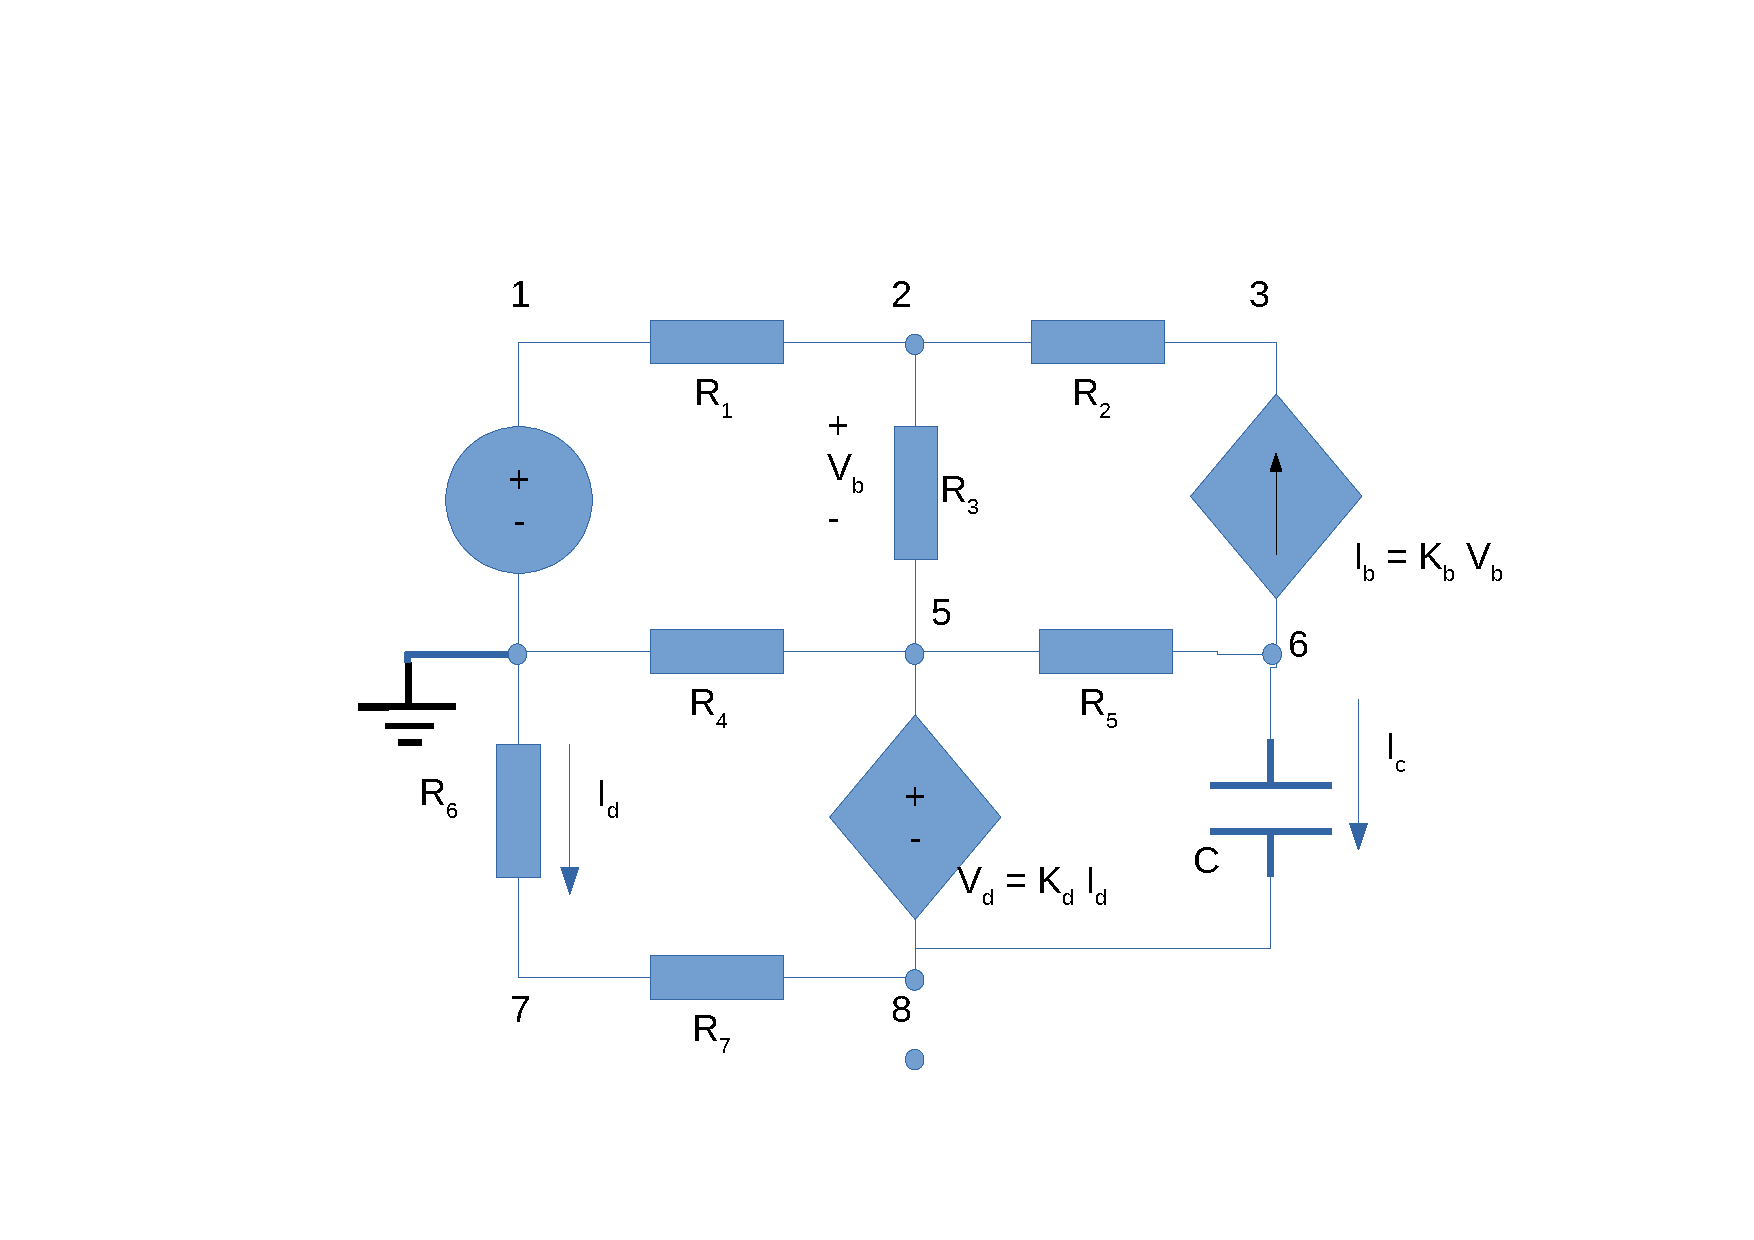
\includegraphics[width=0.8\linewidth]{circuito.pdf}
\caption{Circuit}
\label{fig:circuit}
\end{figure} 
We wrote a system of equations for each theoretical analysis, from Kirchhoff and Ohm's Laws. To get the solutions and plots for these analysis, we used \textit{octave}, which solved our systems of equations efficiently and gave us all currents and voltages for all branches. We then used \textit{ngspice} to get a simulation of this circuit, expecting to obtain the same results. We compared the results from different methods in the conclusion (Section ~\ref{sec:conclusion}).


\section{Mesh Analysis}
\label{sec:mesh analysis}

In this section, the circuit shown in Figure 1 is analysed theoretically using the Mesh Current Method. This method is based on Kirchhoff's Voltage Law (KVL), which states that the sum of all the potencial differences around the loop must be equal to zero.\\
The first step is to identify the meshes (in this case, there are four) and assign a current variable to each one ($I_1, I_2, I_3, I_4$), using a consistent direction (in the four meshes we chose counterclockwise). This can be seen in Figure ~\ref{fig:mesh}.\\

\begin{figure}[H] \centering
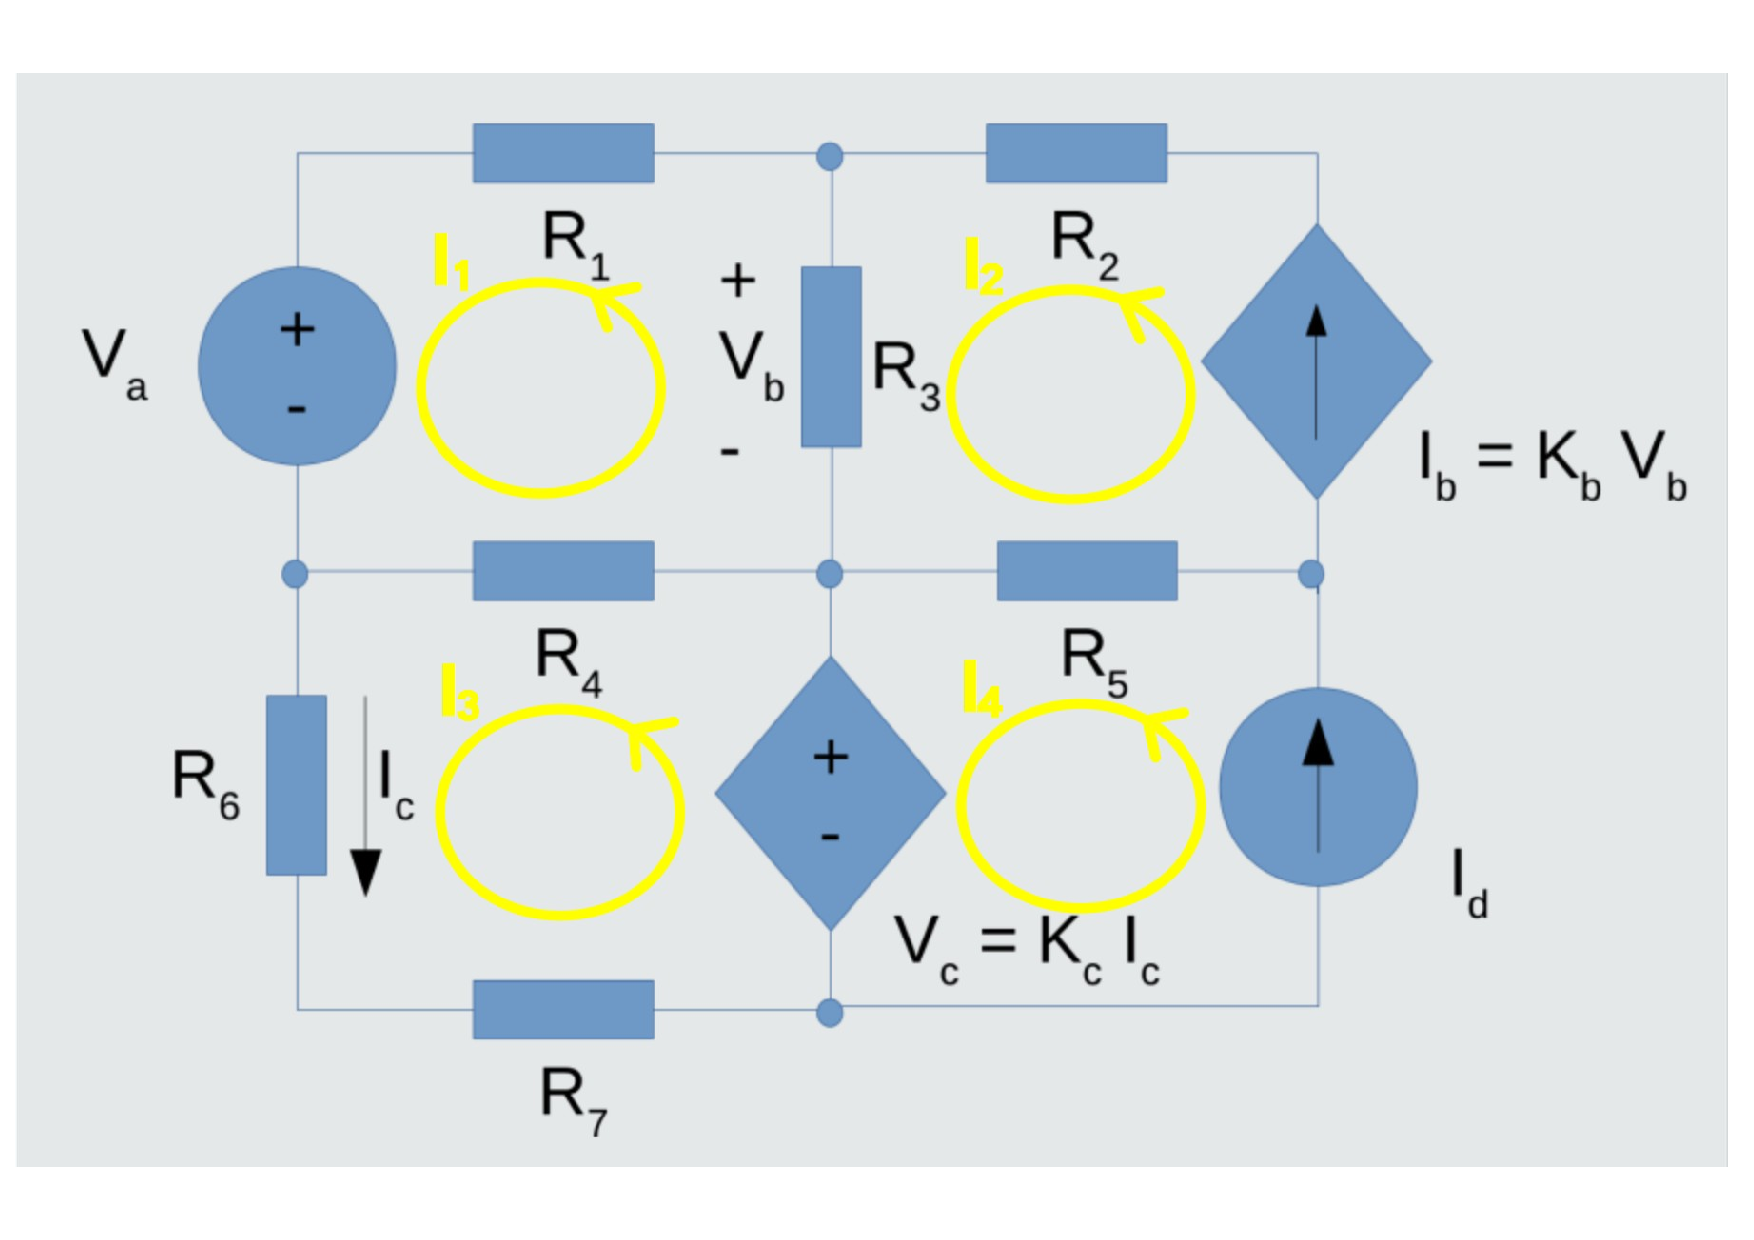
\includegraphics[width=0.7\linewidth]{meshcircuit.pdf}
\caption{Mesh currents}
\label{fig:mesh}
\end{figure}


The second step is to write Kirchhoff's Voltage Law equations around each mesh; however, the value of $I_d$ is already known, so there's no need to write an equation around the fourth mesh. This being said, and knowing by Ohm's Law that
\begin{equation}
  V=RI
\end{equation}

the equation for the first mesh is:

\begin{equation}
  V_a + R_4(I_1 - I_3) + R_3(I_1 - I_2) + R_1I_1 = 0 \Leftrightarrow I_1(R_1+R_3+R_4) - I_2R_3 - I_3R_4 = -V_a
  \label{eq:kvl}
\end{equation}

In the second mesh, noticing that $I_b=I_2$, $V_b$ can be written in two ways:

\[   V_b = \frac{I_2}{K_b}   \]
and
\[   V_b = R_3(I_2-I_1)   \]

Therefore:
\begin{equation}
\frac{I_2}{K_b} = R_3(I_2 - I_1)\Leftrightarrow I_2 = K_bR_3(I_2-I_1)\Leftrightarrow -I_1K_bR_3 + I_2(K_bR_3-1) = 0
  \label{eq:kvl}
\end{equation}

And finally, for the third mesh:
\begin{equation}
  R_6I_3 + R_7I_3 - V_c + R_4(I_3-I_1) = 0
  \label{eq:kvl}
\end{equation}

and since $V_c = K_cI_c$ and $I_c=I_3$:
\begin{equation}
 -I_1R_4 + I_3 (R_4+R_6+R_7-K_c) = 0
  \label{eq:kvl}
\end{equation}

The next step is to solve the resulting system of equations for the mesh currents:

\begin{equation}
\left(\begin{array}{ccc} R_1+R_3+R_4 & -R_3 & -R_4\\ -K_bR_3 & K_bR_3-1 & 0 \\ -R_4 & 0 & R_4+R_6+R_7-K_c \end{array}\right)
\left(\begin{array}{c} I_1 \\ I_2 \\ I_3 \end{array}\right) 
= \left(\begin{array}{c} -V_a \\ 0 \\ 0 \end{array}\right)
\end{equation}


\section{Nodal Analysis}
\label{sec:nodal analysis}

\subsection{Systematic procedure}
In this circuit, there are 8 nodes. Therefore, to solve the circuit we need to find N (number of nodes) -1 equations, which in this case means we must find 7 independent equations. Firstly, we must choose our ground node (node which, by convention, has voltage 0). Typically the node chosen as the ground node is the one that connects to a voltage source so we chose the node that connects the voltage source $V_{a}$ and the resistors 4 and 6. Next, we numbered the remaining nodes as shown in Figure ~\ref{fig:nodes}.

\begin{figure}[ht] \centering
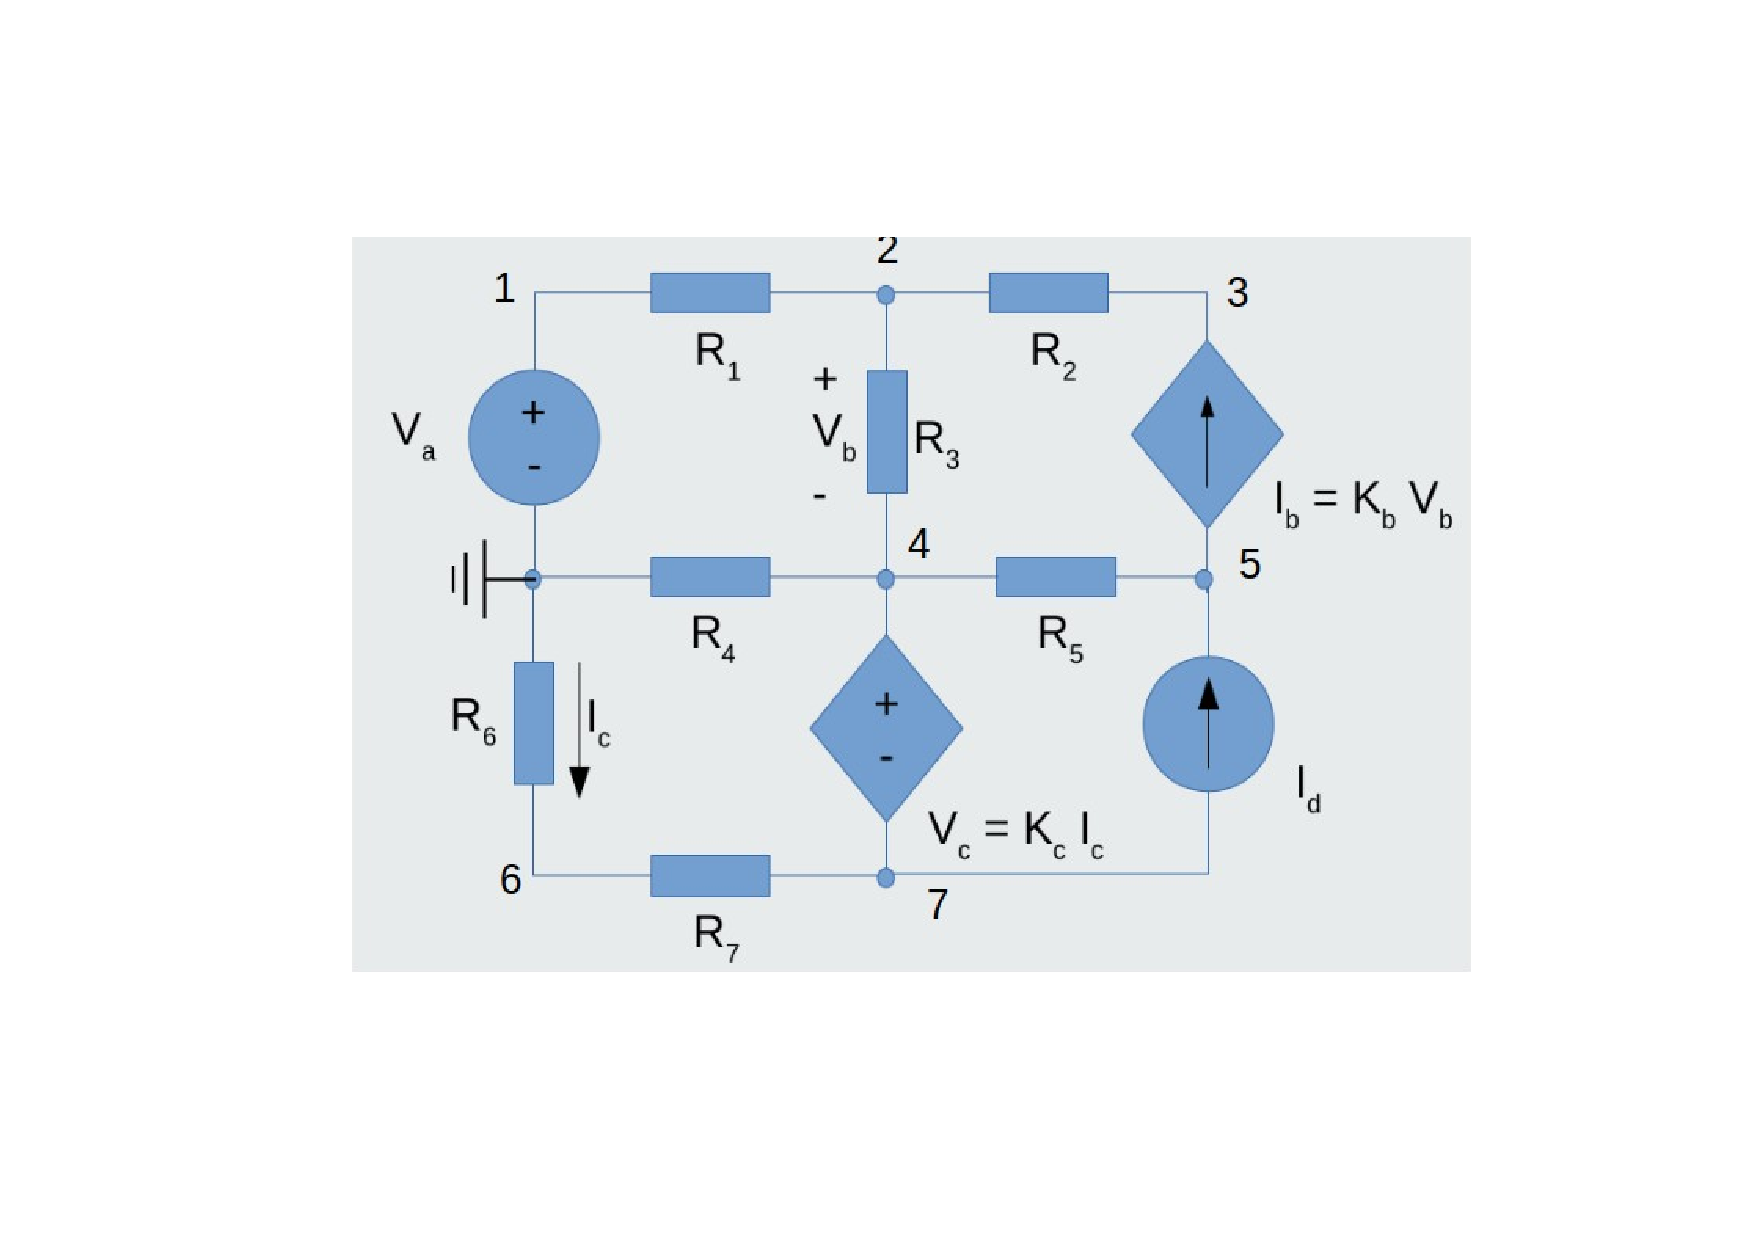
\includegraphics[width=0.8\linewidth]{circuitonodos.pdf}
\caption{Numbered nodes and ground node}
\label{fig:nodes}
\end{figure}
\subsection{Discovering the equations}
Now to discover the equations for each node we need to use Kirchhoff’s Current Law, which states that the sum of all the currents entering and leaving a node must be equal to zero. For simplicity instead of using directly the currents we will also use Ohm's Law. \\
Starting off at node 1, we will consider that current is leaving node 1 towards the voltage source and that current is entering the node from the resistor 1. That leaves us with the following equation:
\begin{equation}
     -i_{a}+\frac{V_{2}-V_{1}}{R_{1}}=0 \Leftrightarrow i_{a}=\frac{V_{2}-V_{1}}{R_{1}},
\end{equation}
where $V_{1}$ and $V_{2}$ are the voltages at nodes 1 and 2 and $i_{a}$ is the current that flows through the voltage source. \\
Moreover, we know the voltage provided by the voltage source is equal to $V_{a}$. Taking into consideration the voltage at the nodes 1 and ground we get:
\begin{equation}
    V_{a}=V_{1}-V_{GND} \Leftrightarrow V_{a}=V_{1}
\end{equation}
where $V_{GND}$ is the voltage at the ground node (by convention = 0).\\
Now looking at node 2. We consider all currents entering the node. From that we get:
\begin{equation}
  \frac{V_{1}-V_{2}}{R_{1}} +\frac{V_{3}-V_{2}}{R_{2}}+\frac{V_{4}-V_{2}}{R_{3}}=0
\end{equation}
Moving along to node 3. Here we have a current that is already named, $I_b$. We consider the current moving as is indicated by the symbol, so entering node 3 and then we also consider that current is leaving node 3 toward the resistor 2. This leaves us with:
\begin{equation}
    I_{b}-\left(\frac{V_{3}-V_{2}}{R_{2}}\right)=0 \Leftrightarrow I_{b}=\frac{V_{3}-V_{2}}{R_{2}}
\end{equation}
Next on the list is node 4. Here we consider that current is leaving the node towards resistor 5 and the current dependant voltage source $V_{c}$ and entering the node from resistors 3 and 4. The KCL equation becomes:
\begin{equation}
    -i_{c}-\left(\frac{V_{4}-V_{5}}{R_{5}}\right)+\frac{V_{2}-V_{4}}{R_{3}}+\frac{V_{GND}-V_{4}}{R_{4}}=0 \Leftrightarrow i_{c}+\frac{V_{4}-V_{5}}{R_{5}}+\frac{V_{4}-V_{2}}{R_{3}}+\frac{V_{4}}{R_{4}}=0 
\end{equation}
where $i_c$ is the current through the current dependant voltage source.\\
From nodes 2, 3 and 4 we can also extract one more equation. Because of the voltage dependant current source and the resistor 3 we know 2 things about $V_{b}$:
\[V_{b}=V_{2}-V_{4} \hspace{5mm} V_{b}=\frac{I_{b}}{K_{b}} \]
Using equation (4) we can further develop this relation between the two equations.
\begin{equation}
    V_{b}=\frac{I_{b}}{K_{b}} \Leftrightarrow V_{b}=\frac{V_{3}-V_{2}}{R_{2} K_{b}} \Leftrightarrow V_{2}-V_{4}=\frac{V_{3}-V_{2}}{R_{2} K_{b}} \Leftrightarrow V_{2}-V_{4}+\frac{V_{2}-V_{3}}{R_{2} K_{b}}=0
\end{equation}
Now onto node 5. We again use the already named voltage dependant current, $I_{b}$ (that is defined in equation 4) and current source $I_{d}$. We define the current direction in accordance with their symbols ($I_{b}$ is leaving the node and $I_{d}$ is entering). We also have a resistor, resistor 5, and we assume current is leaving the resistor and entering the node. 
\begin{equation}
    -I_{b}+I_{d}+\frac{V_{4}-V_{5}}{R_{5}}=0 \Leftrightarrow 
    \frac{V_{3}-V_{2}}{R_{2}}+\frac{V_{5}-V_{4}}{R_{5}}=I_{d}
\end{equation}
The next node is node 6. Here we have a named current entering the node, from resistor 6 called $I_{c}$, and we assume that current is leaving the node towards resistor 7. 
\begin{equation}
    I_{c}-\left(\frac{V_{6}-V_{7}}{R_{7}}\right)=0 \Leftrightarrow 
    \frac{V_{6}-V_{7}}{R_{7}}=I_{c} 
\end{equation}
We also know that
\begin{equation}
   I_{c}=\frac{V_{GND}-V_{6}}{R_{6}}=\frac{-V_{6}}{R_{6}}  
\end{equation}

Combining this with equation (8) we get:
\begin{equation}
    \frac{V_{7}-V_{6}}{R_{7}}-\frac{V_{6}}{R_{6}}=0 
\end{equation}
    The final node is node 7. Here we again come across named current $I_{d}$ and current dependant voltage source $V_{c}$. Current $I_{d}$ is leaving the node and current is entering from the current dependant voltage source and resistor 7. The KCL equation becomes:
    \begin{equation}
     i_{c}+ \frac{V_{6}-V_{7}}{R_{7}}-I_{d}=0 \Leftrightarrow
     i_c+ \frac{V_{6}-V_{7}}{R_{7}}=I_{d}
    \end{equation}
    Since we have common terms we can combine equations (5) and (11) and get:
    \begin{equation}
I_{d}+\frac{V_{7}-V_{6}}{R_{7}}+\frac{V_{4}-V_{5}}{R_{5}}+\frac{V_{4}-V_{2}}{R_{3}}+\frac{V_{4}}{R_{4}}=0 
    \end{equation}
    At this point, we have 7 variables (the voltages at the 7 nodes) and only 6 equations. However, we know that:
    \[ V_c= V_4-V_7 \hspace{5mm} V_c=K_c I_c\]
    Combining this fact with equation (9) we get:
    \begin{equation}
        V_4 -V_7+\frac{K_c V_6}{R_6}=0
    \end{equation}
The next step is to solve the system of equations resulting from equatios 2, 3, 6, 7, 10, 12 and 13 for the node voltages:

    \begin{equation}
\left(\begin{array}{ccccccc} 
1 & 0 & 0 & 0 & 0 & 0 & 0\\
\frac{1}{R_1} & -\frac{1}{R_1}-\frac{1}{R_2} -\frac{1}{R_3} & \frac{1}{R_2} & \frac{1}{R_3}& 0 & 0 & 0 \\
0 & 1+\frac{1}{R_2 K_b} & -\frac{1}{R_2 K_b} & -1 & 0 & 0 & 0 \\
0 & -\frac{1}{R_3} & 0 & \frac{1}{R_3} +\frac{1}{R_4}+\frac{1}{R_5} & -\frac{1}{R_5} & -\frac{1}{R_7} & \frac{1}{R_7} \\
0 & -\frac{1}{R_2} & \frac{1}{R_2} & -\frac{1}{R_5} & \frac{1}{R_5} & 0 & 0 \\
0 & 0 & 0 & 0 & 0 & -\frac{1}{R_6}-\frac{1}{R_7} & \frac{1}{R_7} \\
0 & 0 & 0 & 1 & 0 & \frac{K_c}{R_6} & -1 \\
\end{array}\right)
\left(\begin{array}{c} V_1 \\ V_2 \\ V_3 \\ V_4 \\ V_5 \\ V_6 \\ V_7 \end{array}\right) 
= \left(\begin{array}{c} V_a \\ 0 \\ 0 \\-I_d \\I_d \\ 0 \\0 \end{array}\right)
\end{equation}

\section{\textit{Octave} Results}
Putting both systems of equations in \textit{Octave}, we get the solutions for mesh currents in the first case, and node voltages in the second. From this and Ohm's law we get the following tables for resistors' voltages and currents. The last two lines of both tables pertain to the dependent sources, where $V_c$ refers to the current dependent voltage source and $I_b$ to the voltage dependent current source.


 \subsection{Mesh Analysis}

Solution (mA):
$ \left(\begin{array}{c} I_1 \\ I_2 \\ I_3  \end{array}\right) = \left(\begin{array}{c} -0.233449 \\ -0.244673 \\ 0.992188 \end{array}\right) $
 \begin{table}[H]
 \footnotesize
 \centering
 \caption{Mesh Analysis results}
 \label{tab:tables}
 \begin{center}
 \begin{tabular}{ccc} 
 & Voltage (V) & Current (mA) \\ 
 \hline 


 \hline 
 $R_1$ & -0.239529 & -0.233449 \\ 
 \hline 
 $R_2$ & -0.498337 & -0.244673 \\ 
 \hline 
 $R_3$ & -0.034777 & -0.011224 \\ 
 \hline 
 $R_4$ & -5.028594 & -1.225637 \\ 
 \hline 
 $R_5$ & -4.050308 & -1.290879 \\ 
 \hline 
 $R_6$ & 2.004013 & 0.992188 \\ 
 \hline 
 $R_7$ & 1.030260 & 0.992188 \\ 
 \hline 
 $V_c$ & 8.062868 & 0.992188 \\ 
 \hline 
 $I_b$ & -0.034777 & -0.244673 \\ 
 \hline 
 \end{tabular} 
 \end{center} 
 \end{table}

 \subsection{Nodal Analysis}

Solution (V):
$ \left(\begin{array}{c} V_1 \\ V_2 \\ V_3 \\ V_4 \\ V_5 \\ V_6 \\ V_7 \end{array}\right)= \left(\begin{array}{c} 5.233347 \\ 4.993818 \\ 4.495481 \\ 5.028594 \\ 9.078902 \\ -2.004013 \\ -3.034274 \end{array}\right) $
 \begin{table}[H]
 \footnotesize
 \centering
 \caption{Nodal Analysis results}
 \label{tab:tables}
 \begin{center}
 \begin{tabular}{ccc} 
 & Voltage (V) & Current (mA)\\ 
 \hline 


 \hline 
 $R_1$ & -0.239529 & -0.233449 \\ 
 \hline 
 $R_2$ & -0.498337 & -0.244673 \\ 
 \hline 
 $R_3$ & -0.034777 & -0.011224 \\ 
 \hline 
 $R_4$ & -5.028594 & -1.225637 \\ 
 \hline 
 $R_5$ & -4.050308 & -1.290879 \\ 
 \hline 
 $R_6$ & 2.004013 & 0.992188 \\ 
 \hline 
 $R_7$ & 1.030260 & 0.992188 \\ 
 \hline 
 $V_c$ & 8.062868 & 0.992188 \\ 
 \hline 
 $I_b$ & -0.034777 & -0.244673 \\ 
 \hline 
 \end{tabular} 
 \end{center} 
 \end{table} 


\section{Simulation}
\label{sec:simulation}
In this circuit, we have a current dependent voltage source between nodes 5 and 8, so that, to sense the controlling current, $I_d$, between nodes GND and 7, we need to use a voltage source of voltage 0V, to sense said current. For this purpose, we placed this source between node 7 and a new node - node 9-, which connects the negative terminal of the voltage source and resistor 7, so that it is in series with resistor 6, through which $I_d$ flows, and therefore senses that same current.\\
\subsection{Operating Point Analysis for t\textless0}
To simulate the response of the circuit for t\textless0, where the voltage source introduces to the circuit a constant voltage, $V_s$, the current through the capacitor is zero, so there is an open circuit between nodes 6 and 8. The results of the operating point analysis for this circuit, t\textless0, obtained using \textit{ngspice}, can be seen in Table (ref).\\

\subsection{Operating Point Analysis for t=0}
To get the operating point analysis for t=0, knowing $v_s(0)=0$, we substitute the capacitor, between nodes 6 and 8, with a voltage source $V_x=V_6-V_8$, where $V_6$ and $V_8$ are the voltage for nodes 6 and 8, respectively, obtained in the previous op analysis (for t\textless0). This is needed so continuity of voltage in the capacitor is guaranteed. The results of this analysis, using \testit{ngspice} can be seen in Table (ref).\\
\subsection{Transient Analysis for Natural Response}
From now on, we have a capacitor in its place, between nodes 6 and 8.\\
To simulate the natural response of the circuit, the source $V_s$ was turned off(the voltage has to be 0V to get the natural response), and we used boundary conditions of $V_6$ and $V_8$(voltages in nodes 6 and 8), as the values obtained in t=0. These conditions will also be used in the latter sections. We did transient analysis, for the [0,20]ms time interval, with a 0.02ms time step. The plot of $v_{6}(t)$ is shown in Figure(ref).\\
\subsection{Analysis of Total Response}
For this section, we now have $V_s$ as a sine wave of frequency f=1k Hz, and amplitude 1 ($V_s=sin(2\pi f t)$). A transient analysis was done, for nodes 6 (V6) and 1 (Vs),again for the [0,20]ms time period with a 0.02ms time step. We can then see the results of the voltage introduced to the circuit (Vs) and the total response on node 6, from both this stimulus from Vs and the natural response of the system. This can be seen in Figure (ref).\\
\subsection{Frequency Analysis}
To evaluate the circuit when the frequency changes, we used ac analysis, by decades - using a frequency logscale. Frequencies were considered from 0.1 Hz to 1MHz and we used 100 points to plot both the magnitude and phase of voltages of nodes 1, 6 and of the capacitor $v_c$, which corresponds to $V_6 - V_8$, as functions of frequency. The magnitude plot can be seen in Figure (ref), and the phase plot in Figure (ref).\\


\section{Conclusion}
\label{sec:conclusion}
In this laboratory assignment, the objective of analysing the RC circuit has been achieved. \\
When looking at the tables of currents and voltages obtained by \textit{Octave} and \textit{ngspice} for the analysis of the circuit when t\textless 0 we can that they perfectly match, which is expected since all components considered are linear.\\
In the analysis for t=0, just one voltage is different than 0, $V_6$, and both methods resulted in the same value for this voltage, and for the current that goes throught $R_5$. In the \textit{ngspice} simulation the rest of voltages, that were supposed to be zero (and were, in the table obtained by \textit{Octave}), are in fact values of very small order of magnitude being practically negligible, which checks out.\\
In terms of all of the plots, the ones obtained by \textit{Octave} were a perfect match for the ones obtained in \textit{ngspice}.\\
Only the magnitude plot regarding $V_6$ had differences, when comparing both tools, since they seem to be mirrored.

%\cleardoublepage

% ----------------------------------------------------------------------
%  Bibliography
% ----------------------------------------------------------------------
%\addcontentsline{toc}{section}{\bibname}
%\bibliographystyle{abbrvunsrtnat} % <<<<< SELECT IF USING REFERENCES BY NUMBER (CITATION ORDER)
%\bibliography{../../../BIBfile.bib}

% ----------------------------------------------------------------------
\end{document}
% ----------------------------------------------------------------------

